Para poder recopilar la información de un router, es muy importante tener acceso al mismo mediante el uso de un protocolo de acceso, ya sea telnet, ssh, entre otros, ya que, en caso de no existir el archivo de configuración, es importante crear el mismo mediante la línea de comandos, pero al tratarse de una red, no siempre se tiene acceso físico a todos los dispositivos, por ello la importancia de poder acceder a los mismos.\newline
La herramienta realizada, antes de poder extraer el archivo de configuración, primero se encarga de sobreescribirlo con la configuración actual del router. Para lograr lo anterior, fue necesario utilizar la librería telnetlib, para que, con ayuda de la misma, se puedan ejecutar los comandos necesarios para habilitar el router y generar el archivo con la configuración más actual.\newline
En la siguiente imagen se muestra el código fuente del programa que realiza dicha conexión, así como la ejecución de los comandos.

\pagebreak
\begin{figure}[htbp!]
	\centering
		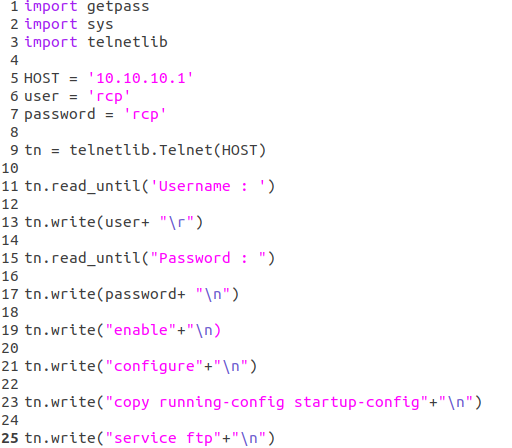
\includegraphics[width=0.8\textwidth]{desarrollo/tarea3/imagenes/imagen1.png}
	\caption{Código fuente para acceder a un router remoto vía Telnet.}
\end{figure}

Para la exportación e importación de los archivos de configuración, se desarrolló un pequeño programa que se encarga de importar el archivo de configuración del router dada su ip, así como de enviar un archivo de configuración seleccionado y reemplazar el archivo “startup-config” de dicho router para cambiar su configuración. La interfaz gráfica se muestra en la siguiente figura.

\begin{figure}[htbp!]
	\centering
		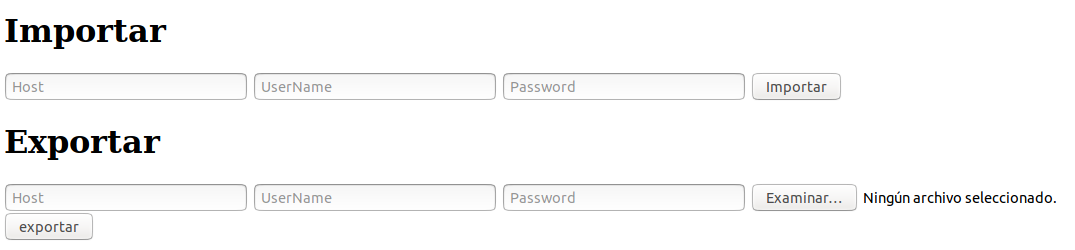
\includegraphics[width=0.8\textwidth]{desarrollo/tarea3/imagenes/imagen2.png}
	\caption{Pantalla principal de la herramienta de importación y exportación de archivos de configuración.}
\end{figure}

Para el punto anterior, se realizaron algunas pruebas de la extracción de los archivos de configuración. Para ello, se utilizó una máquina virtual de Ubuntu dentro de GNS3, así como tres enrutadores, tal como se muestra en la siguiente figura.

\pagebreak
\begin{figure}[htbp!]
	\centering
		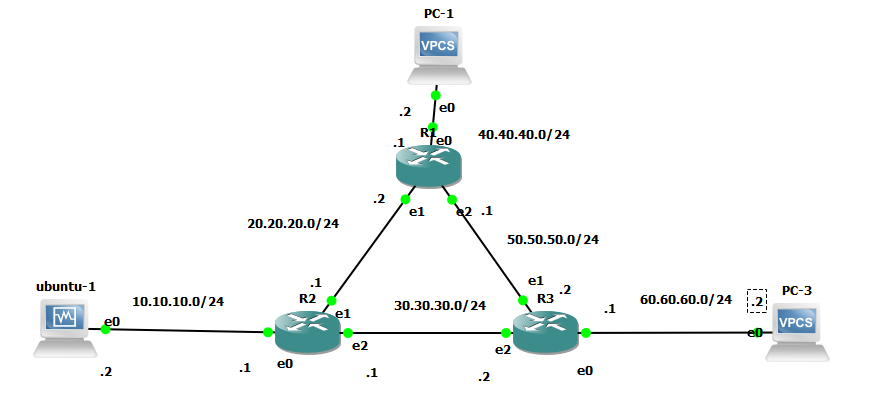
\includegraphics[width=0.8\textwidth]{desarrollo/tarea3/imagenes/imagen3.png}
	\caption{Topología de prueba para la extracción y envío de archivos de configuración.}
\end{figure}

Tras haber realizado la configuración de los routers, se muestra la tabla de enrutamiento de cada uno de ellos. Cabe mencionar que por cuestiones prácticas fueron configurados con el protocolo RIP.

\begin{figure}[htbp!]
	\centering
		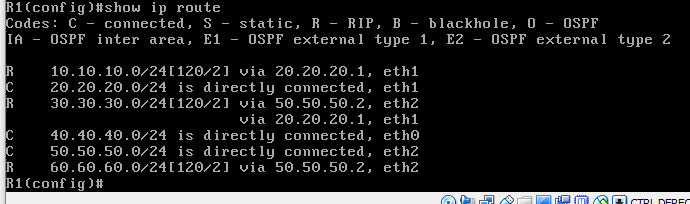
\includegraphics[width=0.8\textwidth]{desarrollo/tarea3/imagenes/imagen4.png}
	\caption{Tabla de enrutamiento del router R1}
\end{figure}

\pagebreak
\begin{figure}[htbp!]
	\centering
		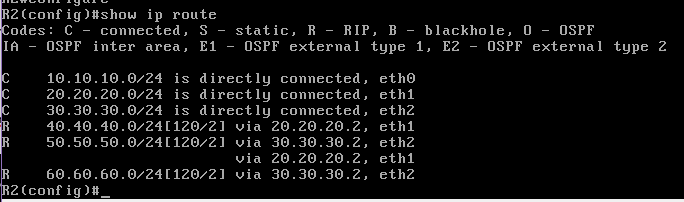
\includegraphics[width=0.8\textwidth]{desarrollo/tarea3/imagenes/imagen5.png}
	\caption{Tabla de enrutamiento del router R1}
\end{figure}

\begin{figure}[htbp!]
	\centering
		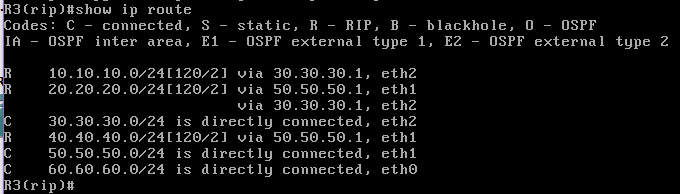
\includegraphics[width=0.8\textwidth]{desarrollo/tarea3/imagenes/imagen6.png}
	\caption{Tabla de enrutamiento del router R1}
\end{figure}

Tras haber verificado la conectividad dentro de la red, se procedió a extraer el archivo de configuración de router. En la siguiente figura se puede observar los datos requeridos en el sistema para poder extraer dicho archivo. Cabe mencionar que solo es necesario especificar la ip de alguna de las interfaces del router, por lo cual, si un router tiene más de una conexión, se podrá acceder al mismo usando distintas direcciones ip.

\begin{figure}[htbp!]
	\centering
		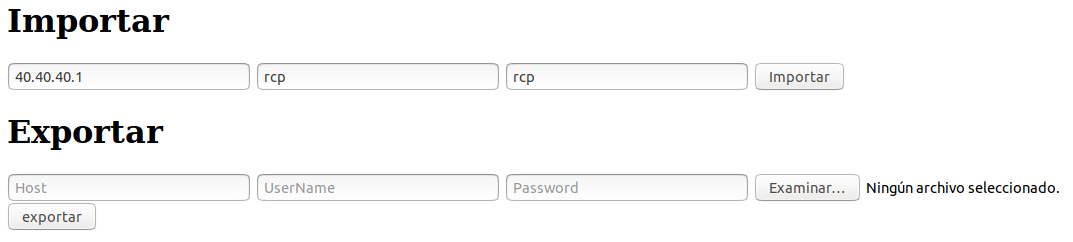
\includegraphics[width=0.8\textwidth]{desarrollo/tarea3/imagenes/imagen7.png}
	\caption{Datos de entrada para la extracción de un archivo de configuración de un router específico.}
\end{figure}

\pagebreak
Una vez realizado lo anterior, se habrá generado un archivo de texto, el cual contiene toda la configuración del router como se muestra en la siguiente figura.

\begin{figure}[htbp!]
	\centering
		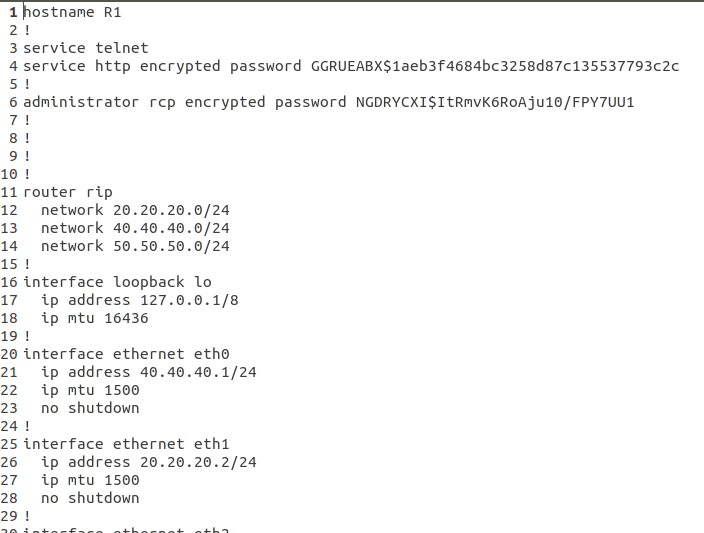
\includegraphics[width=0.8\textwidth]{desarrollo/tarea3/imagenes/imagen8.png}
	\caption{Contenido del archivo de configuración extraído del router R1.}
\end{figure}

Para probar la exportación de los archivos de configuración, se cambió el nombre del host por “PruebaEnvio”. La herramienta permite elegir un archivo desde la computadora, de forma que no es necesario escribir la ruta de dicho archivo. En la siguiente figura se puede observar los datos de entrada para el envío de un archivo de configuraciones hacia un router.

\begin{figure}[htbp!]
	\centering
		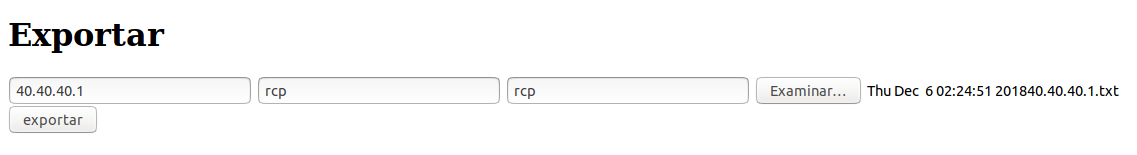
\includegraphics[width=0.8\textwidth]{desarrollo/tarea3/imagenes/imagen9.png}
	\caption{Datos de entrada para la sobreescritura de un archivo de configuraciones de un router.}
\end{figure}

\pagebreak
Finalmente, para verificar que el archivo se recibió correctamente, basta con reiniciar nuestro router y ver que el nombre del host se modificó de forma exitosa.

\begin{figure}[htbp!]
	\centering
		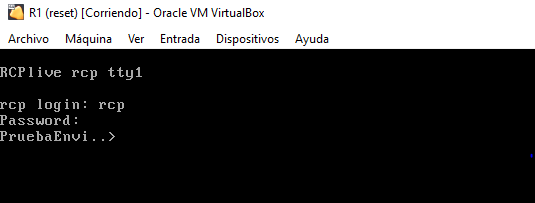
\includegraphics[width=0.8\textwidth]{desarrollo/tarea3/imagenes/imagen10.png}
	\caption{Verificación de los cambios realizados al archivo de configuraciones extraído previamente.}
\end{figure}

Como última parte, se muestra el código fuente de la herramienta que se encarga de la importación y exportación de los archivos de configuración.

\pagebreak
\begin{figure}[htbp!]
	\centering
		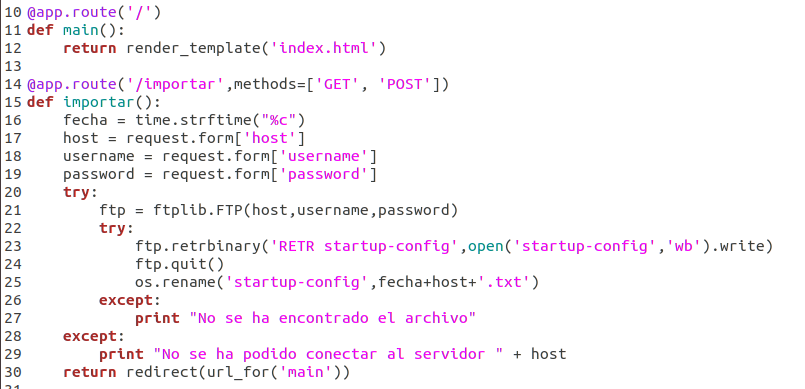
\includegraphics[width=0.8\textwidth]{desarrollo/tarea3/imagenes/imagen11.png}
	\caption{código fuente de la función que extrae el archivo de configuraciones de algún router.}
\end{figure}

\begin{figure}[htbp!]
	\centering
		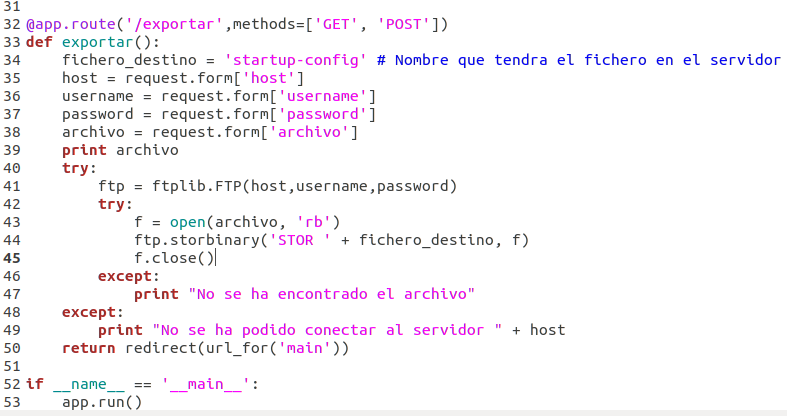
\includegraphics[width=0.8\textwidth]{desarrollo/tarea3/imagenes/imagen12.png}
	\caption{Código fuente de la función que sobreescribe un archivo de configuraciones de algún router.}
\end{figure}































